\documentclass{article}
\usepackage[utf8]{inputenc}

\title{Lesson 5 - Computer Organization}
\author{Matt Chung}
\date{July 18 2017}
\usepackage{amsfonts}
\usepackage{ulem}
\usepackage{amsmath}
\usepackage{tikz}
\usepackage{graphicx} 
\usetikzlibrary{calc}

\begin{document}

\maketitle

\section{}
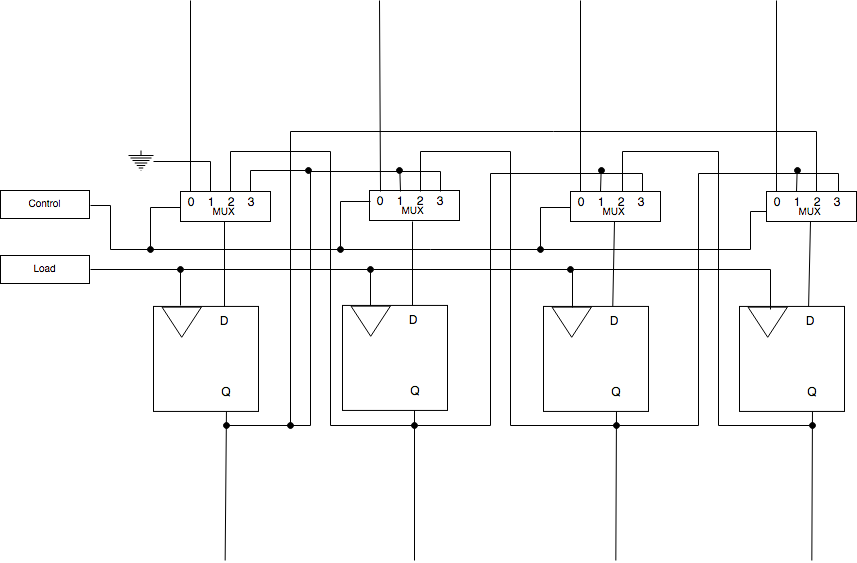
\includegraphics[scale=.50]{q1}

\section{}
\section{}
Despite the drawback of requiring to be refreshed, dynamic RAM is preferred over static memory for a several reasons. To store a single bit, static memory requires four gates: (2) NOR and (2) AND gates. This is insufficient, compared to dynamic RAM, which requires a single capacitor, allowing us to squeeze in more memory—four times as much—on our system.
\section{}
\section{}


\end{document}